% Hier wird der theoretische Teil vorgenommen. 

\chapter{Stand der Technik}

Die zur Erreichung der in \autoref{sec:motivation} definierten Ziele nötigen Grundlagen der Technik sind 
in diesem Kapitel beschrieben. Hierfür bietet \autoref{sec:state-of-the-art-overview}
\textit{\nameref{sec:state-of-the-art-overview}}
zunächst eine Übersicht der in diesem Kapitel beschriebenen Inhalte, um deren Bedeutung besser zu verstehen. 

\section{Übersicht} \label{sec:state-of-the-art-overview}

\begin{figure}[h]
	\centering
	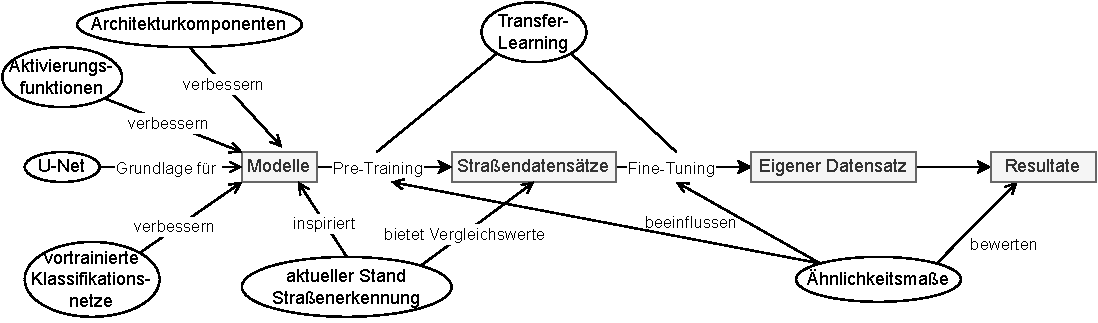
\includegraphics[width=1.\textwidth]{Bilder/overview-background.drawio.pdf} 
	\caption{Überblick über die relevanten Inhalte des Kapitels und wofür diese wichtig sind. Zentral sollen Modelle 
	ausgewählt werden, die dann auf dem Straßendatensatz vortrainiert werden, um daraufhin 
	auf dem eigenen Datensatz trainiert zu werden. Abschließend werden die Resultate mit weiteren Datensätzen bewertet.}
	\label{fig:overview-background}
\end{figure} 

\autoref{fig:overview-background} zeigt eine Übersicht über die in diesem Kapitel relevanten Inhalte und wie diese 
zusammenspielen. Dabei nehmen die zentralen vier Kästen eine besondere Rolle ein: Sie beschreiben das grundsätzliche 
für diese Arbeit geplante Vorgehen, um zu einem guten Ergebnis für die Radwegerkennung zu gelangen. 
\begin{enumerate}
	\item Es werden verschiedene Modelle mit verschiedenen Architekturen erstellt, die dann
	\item auf den Datensätzen, die zur Straßenerkennung zur Verfügung stehen, trainiert werden, um mit diesem Pre-Training
	\item auf dem Datensatz zur Radwegerkennung, der in dieser Arbeit erstellt wird, trainiert zu werden.
	\item Schließlich werden die Ergebnisse bewertet, diskutiert und die unterschiedlichen Modelle und Methoden miteinander verglichen.  
\end{enumerate}
Um die spätere Konzeption der Modelle verstehen zu können, müssen einige Grundlagen im Bereich von verschiedenen 
Architekturkomponenten, Aktivierungsfunktionen, Netzarchitekturen, wie U-Nets oder Klassifikationsnetze, und 
weiteren Elementen, die die Performance verbessern können, gelegt werden. 
Außerdem wird Transfer-Learning und unterschiedliche Methoden dafür aus der Literatur erörtert, um von den 
großen Datensätzen zur Straßenerkennung für die Radwegerkennung profitieren zu können. 
Hierfür wird auch der aktuelle Stand bei der Straßenerkennung untersucht, da die Domäne sehr verwandt zur Radwegerkennung ist.
Weiter werden Ähnlichkeitsmaße untersucht, die zum einen für das Training relevant sind, aber auch für die 
abschließende Bewertung der Resultate.  \\
Zunächst werden allerdings Grundlagen zu neuronalen Netzen und dem Maschinellen Lernen, 
sowie die unterschiedlichen Aufgabenkategorien der Computer-Vision untersucht, sodass die vorher angeführten Themen 
besser zu verstehen sind.  

\section{Grundlagen Neuronale Netze}

Ein \ac{NN} ist eine Sammlung an Architekturen im \ac{ML}, wobei für alle gilt,
dass sie aus mehreren einzelnen \textit{Neuronen} bestehen, die miteinander in Verbindung stehen.
Der Aufbau eines Neurons lässt sich \autoref{fig:neuron} entnehmen.
Die Ausgänge der Neuronen sind mit denen der nächsten Schicht verbunden.
Die einzelnen Eingänge können über Parameter gewichtet einfließen.
Zusätzlich gibt es bei jedem Neuron einen Bias, der gesetzt werden kann.
Das Training eines \ac{NN} besteht darin, optimale Werte der Gewichte zu finden, damit korrekte Schlüsse durch das Netz gezogen werden.
Hierfür wird eine Unterteilung des vorhandenen Datensatzes in Training-, Test- und Validation-Set vorgenommen.

\begin{figure}
	\centering
	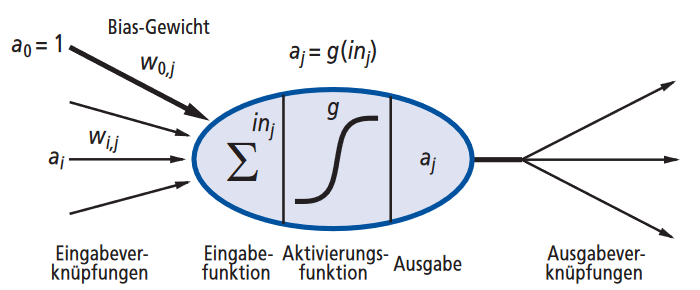
\includegraphics[width=0.65\textwidth]{Bilder/Modell eines Neurons.png} 
	\caption{Modell eines Neurons \cite{Russell.2012}.}
	\label{fig:neuron}
\end{figure} 

\subsection{Training eines neuronalen Netzes}

Für das Training werden Daten aus dem Trainingssatz als Eingabe für das \ac{NN} verwendet.
Die Output-Aktivierung einer Einheit $i$ mit Aktivierungsfunktion $g$ lässt sich mithilfe von \autoref{eq:activationNeuron} bestimmen:
\begin{align}
	\label{eq:activationNeuron} a_j = g(\sum_{i = 0}^{n}w_{i,j} \cdot a_i) ~.
\end{align}
Die Aktivierungsfunktion bestimmt den Grad der Aktivierung $a_j$, also den numerischen Wert, den das nachfolgende Neuron erhält.
Der errechnete Output der letzten Aktivierung wird mit dem erwarteten Ergebnis verglichen.
Die Anpassung der Gewichte erfolgt anschließend über Backpropagation.
Hierbei werden die Fehler der Ausgabeneuronen auf jedes vorherige Neuron zurückgeführt.
Die für die Aktualisierung genutzte Lernrate entscheidet darüber, wie schnell eine Anpassung der Gewichte erfolgt.
Sie kann im Laufe des Trainings verringert werden, um die Parameter feingranular anzupassen.

Das \ac{NN} wird mithilfe der Testdaten bewertet, die Validierungsdaten können für eine Hyperparameter-Anpassung während des Trainings
verwendet werden. Das Training verläuft in Epochen, wobei eine Epoche das Durchlaufen aller Trainingsdaten meint. 
Es folgen so viele Epochen, wie vorgegeben, oder bis sich das Netz nicht mehr verbessert. Für ein schnelleres Training werden die 
Trainingsdaten in Batches einer bestimmten Größe eingeteilt, die parallel verarbeitet werden können. \\  
Für ein gutes Ergebnis sollten verschiedene Kategorien der Bilder in allen drei Datensets gleichermaßen repräsentiert sein.
Eine Klassen-Imbalance sollte vermieden werden.
Diese liegt vor, wenn eine Klasse deutlich stärker als eine andere vertreten ist, z.B. Hintergrundpixel im Vergleich zu Straßen.
Das \ac{NN} vernachlässigt dann ggf. die unterrepräsentierte Klasse und führt zu schlechteren Ergebnissen.
Die Eingabedaten sollten zusätzlich standardisiert und normalisiert sein, um das Lernen zu beschleunigen. 

Bei der \textit{Ground-Truth} eines Datensatzes handelt es sich um das vorgegebene Ergebnis, mit dem der Output des \ac{NN}	verglichen wird.
Das Ergebnis kann beispielsweise ein Label für eine Klassifizierung sein.
Eine hohe Datenqualität sollte gegeben sein, da die Berechnung der Parameter direkt von der Ground-Truth abhängig ist.

Ist ein Modell zu komplex für die gegebenen Trainingsdaten, kann es zu \textit{Overfitting} kommen. Das bedeutet, 
das Netz lernt die Beispiele auswendig und generalisiert nicht. 
Dem kann entweder mit \textit{Regularisierung} entgegengewirkt werden, welche die Komplexität eines Modells zu reduzieren versucht,
oder mit \textit{Augmentierung} der Eingaben, wodurch ein Auswendiglernen durch unterschiedlichere Eingaben erschwert wird  
\cites{Goodfellow.2016, Russell.2012}.


\subsection{\acf{CNN}}

Ein \ac{CNN} ist eine bestimmte Art eines \ac{NN}.
Zwischen den einzelnen Schichten befinden sich \textit{Convolutional Layers}, auch Faltungsschichten genannt.
Die Faltungsschichten lernen die Merkmalsextraktion, indem sie sogenannte Features mithilfe von Filtern erkennen.
Innerhalb der ersten Schichten handelt es sich häufig um Kantendetektion oder die Ermittlung von einfachen Formen.
Das Ergebnis der Convolutional Layers bilden Feature-Maps.

Um den Fokus auf stark ausgeprägte Features zu legen, können \textit{Pooling Layers} verwendet werden.
Diese verringern die Dimensionen des Outputs, indem sie beispielsweise nur den maximalen Wert eines bestimmten Bereiches an die nächste Schicht weitergeben.
\ac{CNN}s werden bei Bildern eingesetzt, da eine räumliche Beziehung zwischen einzelnen Bildpunkten Berücksichtigung findet, räumlich zusammengehörige Regionen werden verbunden.
Die Pooling-Schichten besitzen im Gegensatz zu den Convolutional-Schichten keine Parameter.
Zu beachten ist, dass das Pooling zu einer räumlichen Invarianz der Merkmale führt.
Über eine voll vermaschte Schicht nach der letzten Convolutional-Schicht kann z.B. eine Klassifikation gelernt werden.
\autoref{fig:LeNet} zeigt ein Beispiel für ein \ac{CNN}.

\begin{figure}
	\centering
	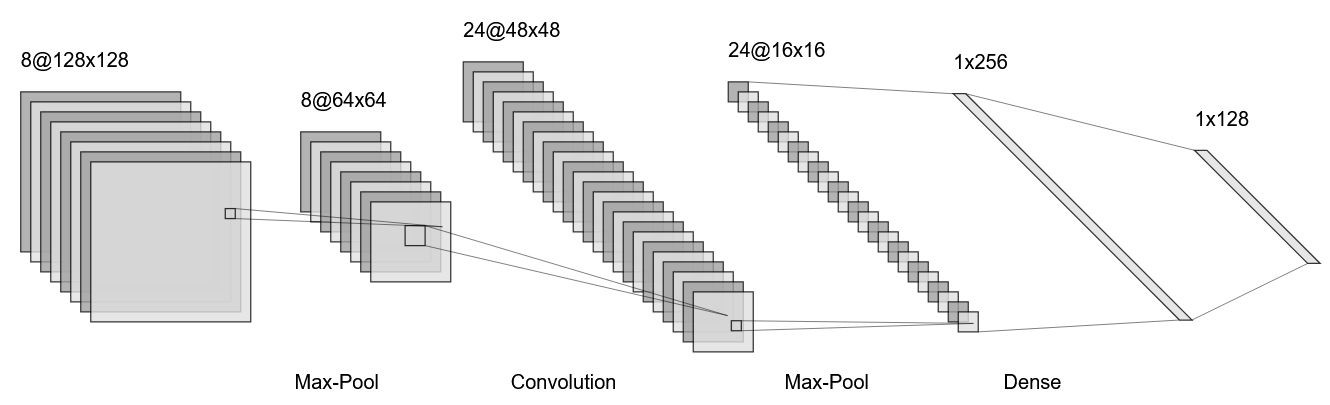
\includegraphics[width=0.8\textwidth]{Bilder/LeNet.png} 
	\caption{LeNet als Beispiel für ein einfaches \ac{CNN}.}
	\label{fig:LeNet}
\end{figure}

\section{Aufgabenkategorien} \label{sec:aufgabenkategorien}
Im Bereich der Computer Vision gibt es verschiedene Problemstellungen, die unterschiedlich gelöst werden können.
Die einzelnen Lösungsansätze werden jeweils einer Aufgabenkategorie zugeordnet.
Nachfolgend wird ein Überblick über die Kategorien \textit{Klassifizierung}, \textit{Object Detection} und \textit{Image Semantic Segmentation} gegeben.
Eine Visualisierung ist in \autoref{fig:categories} gegeben.
Die aufgeführten Kategorien nehmen in der genannten Reihenfolge in ihrer Komplexität zu.

\begin{itemize}
	\item \textit{Klassifizierung:}
	Eine reine Klassifizierung ist die einfachste Lösungskategorie. 
	Es soll lediglich erkannt werden, welche Klasse in einem Bild enthalten ist.
	Die Lokalität des erkannten Objektes wird vernachlässigt, es handelt sich rein umd die Zuordnung zu einer Klasse.
	Dies lässt sich auch entsprechend auf die Erkennung von mehreren Klassen erweitern.
	
	\item \textit{Object Detection:}
	Eine Erweiterung der Klassifizierung um die Lokalität des erkannten Objektes wird Image Localization genannt.
	Für mehrere Objekte wird der Begriff Object Detection verwendet.
	Die Darstellung erkannter Objekte wird über Bounding Boxes realisiert, welche die Objekte jeweils umschließen.

	\item \textit{Semantic Segmentation:}
	Die bei der Object Detection verwendeten Bounding Boxes geben keine Rückschlüsse auf die konkrete Form der Klasse.
	Je nach Lage des Objektes kann nur ein Bruchteil der Bounding Box von der erkannten Klasse gefüllt sein.
	Abhilfe schafft die Verwendung einer pixelweisen Maske anstelle einer Bounding Box, das Objekt kann von seiner Umgebung abgegrenzt werden.

	\item \textit{Instance Segmentation:}
	Zusätzlich zur Semantic Segmentation kann noch gefordert werden, dass einzelne Instanzen verschiedener Objekte 
	unterschieden werden sollen.
	Diese Forderung wird dann als \textit{Instance Segmentation} bezeichnet \cite{Sharma.21.08.2019}.
\end{itemize}

\begin{figure}
	\centering
	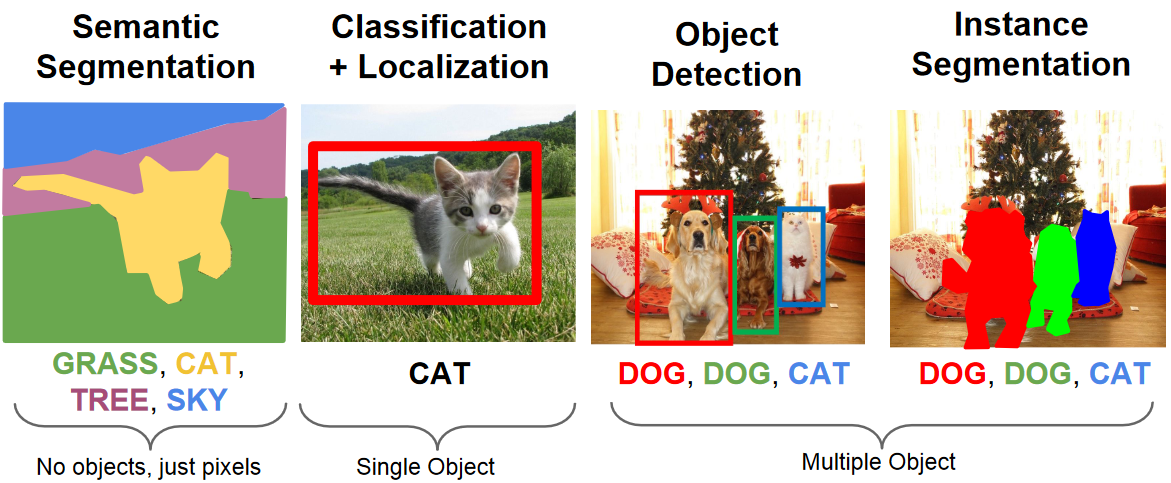
\includegraphics[width=0.8\textwidth]{Bilder/categories.png} 
	\caption{Verschiedene Aufgabenkategorien \cite{.10.11.2022}.}
	\label{fig:categories}
\end{figure} 

\section{Aktivierungsfunktionen} \label{sec:activation}

Im Folgenden wird der Stand der Technik für Aktivierungsfunktionen in \ac{ML}-Modellen dargelegt,
hierzu werden einige Funktionen kurz vorgestellt und deren Vor- und Nachteile bewertet. 

\subsection{Sigmoid}

Die \textit{Sigmoid}-Funktion bildet die Eingabe auf einen Wert im Intervall $(0;1)$ ab und wird durch \autoref{eq:sigmoid} beschrieben.
Der Vorteil hier ist, dass Aktivierungen nie groß werden können, wodurch einzelne Neuronen nicht den Gradienten dominieren können und 
eine fortlaufende Normalisierung durchgeführt wird. Die Probleme hingegen sind, dass die Funktion eher aufwendig zu berechnen ist 
und dass die Ableitung für betragsmäßig größere Werte verschwindet. Hierdurch kann es zum \textit{Vanishing-Gradient-Problem} kommen, wobei 
Neuronen in den flacheren Schichten eines neuronalen Netzes kaum noch upgedated werden \cite{Goodfellow.2016} 
\begin{align}
	\label{eq:sigmoid} Sigmoid(z) = \frac{1}{1+e^{-z}}~.
\end{align} 

\subsection{\acf{ReLU}} \label{sec:activation:relu}

Die \textit{\acf{ReLU}} ist eine Aktivierungsfunktion, welche durch \autoref{eq:relu} ausgedrückt wird. 
\ac{ReLU} ist inzwischen der de-facto Standard von Aktivierungsfunktionen in den verborgenen Schichten eines Deep-Learning-Modells.
Dies liegt vor allem daran, dass das Vanishing-Gradient-Problem adressiert wird. Allerdings hat \ac{ReLU} das Problem, 
dass Neuronen auf $0$ gesetzt werden, wodurch sie kein Gradienten-Update mehr erhalten und dauerhaft genullt bleiben 
und somit nichts mehr zum Netzwerk beitragen - die Neuronen \enquote{sterben}. Das Problem wird \textit{Dying-\ac{ReLU}-Problem} genannt \cite{Goodfellow.2016} 
\begin{align}
	\label{eq:relu} ReLU(z) = \begin{cases} 
		z & z > 0 \\
		0 & z \leq 0 
	\end{cases}~.
\end{align} 

\ac{ReLU} erzielt eine höhere Inferenz- und Trainingsgeschwindigkeit bei gleicher oder besserer Performanz, 
als Sigmoid. Dies liegt zum einen an der Verbesserung des Vanishing-Gradient-Problems und zum anderen an der 
simpleren und damit leichter zu berechnenden Funktion \cite{Goodfellow.2016}.

\subsection{\acf{ELU}} \label{sec:activation:elu}

Die \textit{\acf{ELU}} ist eine Aktivierungsfunktion, die das Dying-\ac{ReLU}-Problem adressieren soll. 
Ausgedrückt wird die Funktion durch \autoref{eq:elu}. Die negative Komponente lässt zu, dass Neuronen nicht 
von einem Satz auf $0$ zurückkommen können, und weiterhin etwas zur Zielfunktion beitragen können. Außerdem ist die mittlere 
Aktivierung näher an $0$ als bei \ac{ReLU}, was zur Folge hat, dass das Training schneller konvergiert \cite{Clevert.23112015}
\begin{align}
	\label{eq:elu} ELU(z) = \begin{cases} 
		z & z > 0 \\
		\alpha \cdot (e^z - 1) & z \leq 0 
	\end{cases} ~.
\end{align}

Sowohl \ac{ReLU} als auch \ac{ELU} haben das Problem, dass Aktivierungen beliebig groß werden können, 
wodurch einige wenige Neuronen den Gradienten dominieren können, was zu langsamen Training und suboptimaler Performanz führen kann. 


\section{Ähnlichkeitsmaße} \label{sec:evaluation-metrics}

Im Folgenden sollen Ähnlichkeitsmaße zwischen Mengen, insbesondere 
solche, die als Kostenfunktion bzw. Bewertungsmetrik für einen binären 
Klassifikator verwendet werden können, untersucht werden. Hierzu wird zunächst Cross-Entropy betrachtet,
gefolgt von dem Dice- bzw. F-Maß. Weiter werden \ac{IoU} und das darauf aufbauende Quality-Maß betrachtet.

\subsection{\acf{BCE}}

Die \textit{Cross-Entropy} (bzw. dt. \textit{Kreuzentropie}) ist ein Maß des Unterschieds zweier
Wahrscheinlichkeitsdistributionen. Im Spezialfall einer binären Wahrscheinlichkeitsvariable 
kann die Cross-Entropy zur \textit{\acf{BCE}} spezialisiert werden, um auf ein binäres 
Klassifikationsproblem angewandt zu werden. 
\autoref{eq:bce} zeigt die Kalkulation von \ac{BCE}, wobei $p \in [0;1]$ die Prediction 
eines binären Klassifikators und $y \in \{0,1\}$ der Wert des Labels darstellen
\begin{align}
	\label{eq:bce} BCE = -[p \cdot \log(y) + (1-p) \cdot \log(1-y) ]~.
\end{align} 
Um über $n$ Prediction-Label-Paare $(p_i; y_i)$ den \ac{BCE} zu berechnen, wird das arithmetische Mittel nach
\autoref{eq:bce-mean} gebildet \cites{Cybenko.1999}{Murphy.2012}
\begin{align}
	\label{eq:bce-mean} BCE = -\frac{1}{n}\sum_{i = 1}^{n}[p_i \cdot \log(y_i) + (1-p_i) \cdot \log(1-y_i) ]~.
\end{align}

\acf{BCE} kann ebenfalls für semantische Segmentierung verwendet werden. So wird \acf{BCE} 
für das originelle U-Net genutzt \cite{Ronneberger.18052015}. 

Aus \autoref{eq:bce-mean} geht hervor, warum \ac{BCE} gut geeignet für Klassifikationsprobleme ist.
Im Gegensatz zum mittleren absoluten Fehler, bei dem ein Fehler linear eingeht, und zum mittleren quadratischen Fehler,
bei dem ein Fehler quadratisch eingeht, geht ein Fehler bei \ac{BCE} exponentiell ein. 
Ein größerer Fehler wiegt also exponentiell stärker als ein kleinerer Fehler. 
Hierdurch werden die Fehler pro Datenpunkt und Klasse sehr klein, 
wodurch gute Performance und gute Generalisierung bei \ac{ML}-Modellen erreicht werden können. \\

Bei stark ungleichmäßiger Klassenverteilung kann es jedoch dazu kommen, 
dass die unterrepräsentierte Klasse kaum noch geschätzt wird, 
da der Fehler einer falsch geschätzten überrepräsentierten Klasse zu stark bestraft wird.
Dadurch lernt der Algorithmus, die unterrepräsentierte Klasse kaum zu schätzen.
Eine Abhilfe dagegen schafft eine Gewichtung der unterschiedlichen Klassen \cite{Ronneberger.18052015}.

\subsection{Dice- und F-Maß}

Das \textit{Dice-} oder auch \textit{Sorensen-Dice-}Maß $D$ wurde 1945 bzw. 1948 erstmals vorgestellt und genutzt, um die Ähnlichkeit zweier botanischer Stichproben zu ermitteln. Verallgemeinert auf diskrete Mengen $X$, $Y$ kann deren Ähnlichkeit nach Dice $D$ beschrieben werden durch \autoref{eq:dice-coeff}. Es gilt $D \in [0; 1]$ \cite{Dice.1945} 
\begin{align}
	\label{eq:dice-coeff} D = \frac{2 \cdot | X \cap Y |}{2 \cdot | X \cap Y | + |Y \setminus X| + |X \setminus Y|} 
	=\frac{2 \cdot | X \cap Y |}{|X| + |Y|} ~.
\end{align} 

Angewandt auf boolesche Mengen und binäre Klassifikatoren ist das Dice-Maß gleich dem $F_1$-Maß, das ein Maß für die Qualität eines statistischen Tests darstellt. Dafür sei $X$ nun die Menge der positiven Elemente und $Y$ die Menge der als positiv eingestuften Elemente. Dann ist die \textit{Genauigkeit} oder auch \textit{Precision} gegeben durch
\begin{align}
	\label{eq:precision} P = \frac{|X \cap Y|}{|Y|}~,
\end{align}
den Anteil der richtig eingestuften Elemente an allen positiv eingestuften Elementen und die \textit{Trefferquote} oder auch \textit{Recall} gegeben durch
\begin{align}
	\label{eq:recall} R = \frac{|X \cap Y|}{|X|}~,
\end{align}
den Anteil der richtig eingestuften Elemente an allen positiven Elementen. \\
Das F-Maß, bzw. genauer das $F_1$-Maß, ist dann gegeben durch das harmonische Mittel aus Precision $P$ und Recall $R$, wobei $tp$ die Anzahl von wahr-positiven, $fp$ die Anzahl von falsch-positiven und $fn$ die Anzahl von falsch-negativen Elementen ist \cite{YutakaSasaki.2007}:
\begin{align}
	\label{eq:f1} F_{1} = \frac{2\cdot P\cdot R}{P + R} = \frac{2\cdot tp}{2 \cdot tp + fp + fn}~.
\end{align}
Precision und Recall können mit einem Faktor $\alpha$ unterschiedlich zueinander gewichtet werden, um mit $F_{\alpha}$ unterschiedliche Aspekte zu fokussieren. 

Das Dice-, bzw. $F_{\alpha}$-Maß kann leicht für eine differenzierbare Kostenfunktion genutzt werden mit Dice-Loss $D_{L}(X, Y) = 1 - D(X,Y)$, bzw. $F_{\alpha}$-Loss $F_{\alpha L}(X,Y) = 1 - F_{\alpha}(X,Y)$. 


\subsection{\acf{IoU}}

Die \textit{\acf{IoU}-} bzw. \textit{Jaccard-Ähnlichkeitsmetrik} ist ein weit verbreitetes Maß zur Bestimmung der Ähnlichkeit zwei diskreter Mengen. Hierzu seien $X$ und $Y$ diskrete Mengen. Dann ist die $IoU$ gegeben durch 
\begin{align}
	\label{eq:iou} IoU = \frac{|X\cap Y|}{|X \cup Y|} = \frac{| X \cap Y |}{| X \cap Y | + |Y \setminus X| + |X \setminus Y|}~.
\end{align} 
Für ein binäres Klassifikationsproblem lässt sich die $IoU$ ausdrücken durch 
\begin{align}
	\label{eq:iou-binary} IoU = \begin{cases}
		1 & tp + fp + fn = 0 \\ 
		\frac{tp}{tp + fp + fn} & else \\
	\end{cases}~,
\end{align}
wobei $tp$, $fp$, $fn$ wie in \autoref{eq:f1} \cite{Fletcher.2018}. 

Auffällig ist die Ähnlichkeit zum Dice- bzw. $F_{1}$-Maß. Es ist allerdings anzumerken, dass bei Dice/$F_1$ die $tp$, also die Wahr-Positiven, stärker gewichtet werden, als bei der \ac{IoU}. Die augenscheinliche Ähnlichkeit lässt sich durch die Beziehungen
\begin{align}
	\label{eq:dice-iou} IoU = \frac{D}{2 - D} \\
	D = \frac{2 \cdot IoU}{1 + IoU} ~,
\end{align}
beschreiben.
Im Gegensatz zur \ac{IoU} wird beim Dice-Maß eine höhere Gewichtung auf die wahr-positiven Elemente 
gelegt.

\subsection{Quality} \label{sec:evaluation-metrics:quality}

Die \textit{Quality} soll einige Probleme der \ac{IoU} beheben, um ein Ähnlichkeitsmaß darzustellen, 
was näher an der praktischen und vom Menschen wahrgenommen Leistung eines \ac{ML}-Modells zur semantischen Segmentierung liegt.
So soll relativiert werden, dass vor allem im Randbereich einer Segmentierung einzelne abweichende Pixel
nicht als falsch anerkannt werden, sodass die Segmentierung im Großen und Ganzen als richtig anerkannt wird. 
Ursprünglich wurde dieses Maß 1998 zur empirischen Bewertung der automatischen Straßenextraktion entwickelt \cite{ChristianWiedemann.1998}. 

Konkret handelt es sich bei der \textit{Quality} um eine gepufferte Form der \ac{IoU},
die toleranter bezüglich der Lokalität der Elemente der verglichenen Mengen, oder konkreter,
der Pixel einer semantischen Segmentierung, ist, 
wobei für dieselbe Eingabe $Quality \geq IoU$; $Quality \in [0;1]$ gilt, abhängig von der Puffergröße. 
Die Puffergröße beschreibt den Radius um $tp$-Elemente, in dem $fp$ und $fn$ noch als $tp$ gelten.   
Die Quality wird analog zur \ac{IoU} über eine gepufferte Precision - die \textit{Correctness} - 
und über einen gepufferten Recall - die \textit{Completeness} - berechnet. Insbesondere werden einige Elemente, 
die zuvor als $fp$ und $fn$ eingeordnet wurden, hiermit zu $tp$ konvertiert.

Bezüglich der \textit{Quality} ist die Puffergröße ein wichtiger Parameter.
Wird diese zu groß gewählt, werden gegebenenfalls positive Pixel, die weit abseits liegen und keinen Radweg andeuten, fälschlicherweise 
als $tp$ erkannt. Wird die Puffergröße zu klein gewählt, wird lediglich eine Toleranz gegenüber ungeraden 
Kanten in der Prediction aufgebaut, nicht aber die Verschiebung des gesamten Radwegs akzeptiert.

In der ursprünglichen Beschreibung der \textit{Quality} wird das Maß auf kontinuierlichen Vektoren anstelle von diskreten Rastern angewandt, wodurch nur die 
Idee, nicht aber die Berechnung auf das konkrete Problem der semantischen Segmentierung angewendet werden kann. Dementsprechend ist es nötig, 
die hier vorgestellte \textit{Quality} auf den spezifischen Anwendungsfall der Radwegerkennung anzupassen, 
was in \autoref{sec:eval:biou} vorgenommen wird. 

\section{Architekturkomponenten}

Im Folgenden werden verschiedene Architekturkomponenten diskutiert, die im \ac{ML} allgemein 
bzw. bei semantischer Segmentierung im Speziellen verwendet werden. Hierzu werden zunächst Dropout-Layer 
und Batch-Normalization-Layer begutachtet. 

\subsection{Dropout} \label{sec:architekturkomponenten:dropout}

\textit{Dropout} ist eine ressourcenschonende Regularisierungstechnik für \ac{ML}-Modelle. 
Hierbei werden einzelne Neuronen mit einer Wahrscheinlichkeit von \textit{Rate} $r$ während des Trainings 
deaktiviert, also deren Output auf $0$ gesetzt \cites{Goodfellow.2016}{NitishSrivastava.2014}. \\s
Es hat sich gezeigt, dass Dropout eine effektivere Regularisierungstechnik zur Minderung von Overfitting ist, 
als andere ressourcenschonende Techniken, wie \textit{Weight-Decay}, \textit{Filter-Norm-Constraints} oder 
\textit{Sparse-Activity-Regularization}, wobei Dropout für eine noch bessere Regularisierung mit diesen kombiniert werden kann \cites{Goodfellow.2016}.

\subsection{Batch-Normalization} \label{sec:architekturkomponenten:batchnorm}

\textit{Batch-Normalization} normalisiert und standardisiert den Output von Neuronen auf Basis des Mittelwerts 
und der Streuung einer Batch während des Trainings. Für die Inferenz werden Durchschnittswerte 
des Mittelwerts und der Streuung der Batches des Trainingsdatensatzes herangezogen und angewandt. \\
Batch-Normalization führt zu einer schnelleren Konvergenz im Training, 
sodass die Anzahl an benötigten Epochen in manchen Fällen halbiert werden kann. Des Weiteren führt 
Batch-Normalization zu einer gewissen Regularisierung, da es die Kostenfunktion zu einem bestimmten Grad glättet 
\cites{Goodfellow.2016}{Ioffe.11022015}.
Besonders gut funktioniert Batch-Normalization für \acp{CNN} und Netzwerke mit Sigmoid-Aktivierungsfunktion
\cites{Goodfellow.2016}.

\section{U-Net} \label{sec:architekturkomponenten:unet}

Die \textit{U-Net-Architektur} beschreibt eine \textit{Fully-Convolutional-Network-Architektur}, die erstmals in Freiburg 2015 vorgestellt wurde 
und herausragende Ergebnisse für verschiedene Benchmarks, insbesondere zur semantischen Segmentierung kleiner Datensätze, liefert. \\
Aus \autoref{fig:u-net-architecture} geht die namensgebende Architektur des U-Net hervor. Die folgenden Besonderheiten 
führen zu der sehr guten Performanz des Netzes bei semantischer Segmentierung \cite{Ronneberger.18052015}:
\begin{itemize}
	\item Das Netz besteht aus einem kontrahierenden Encoder-Teil (linke Hälfte) und einem expandierenden und symmetrisch aufgebauten
	Decoder-Teil (rechte Hälfte). Der Encoder erzeugt feinere \textit{Feature-Maps} mit zunehmender Netztiefe, 
	während der Decoder diese wieder extrapoliert, was zu einer besseren Lokalisierung führt. 
	\item Zwischen den jeweiligen symmetrischen Encoder- bzw. Decoder-Blöcken befinden sich \textit{Skip-Connections}\footnote{\textit{copy and crop} in der Abbildung.}.
	Zusammen mit dem vorherigen Punkt erhöht dies weiter die Lokalisierung und Performanz, da der jeweilige Decoder-Block feinere Features von der \textit{Up-Convolution}\footnote{implementiert als \textit{Transposed Convolutions}.},
	wie auch den größeren Kontext von früheren Blocks mittels Skip-Connection erhält. 
	\item Zur Mitte des Netzes hin erhöht sich die Anzahl der Convolution-Filter und damit die Anzahl der \textit{Channel}, 
	während sich die Dimensionen der einzelnen Feature-Maps durch das \textit{Downsampling} verringert. 
	Hierbei ist anzumerken, dass bei der Implementation kein \textit{Padding} für die Convolutions verwendet wird,
	wodurch sich die Dimensionen der Feature-Maps nach jeder Convolution verringert. 
	Hieraus folgt ein Zuschneiden für die Skip-Connections. 
\end{itemize}

Im originalen U-Net beginnt der erste Convolutional-Block mit 64 Filtern, welche
sich blockweise bis zum Mittel-Block verdoppeln, der dann 1024 Filter
besitzt. Daraufhin halbieren sich die Filter mit jedem weiteren Decoder-Block
wieder.
Das U-Net hat ca. 24 Mio. Parameter. \\
Ein Problem, welches im ursprünglichen U-Net-Paper erwähnt wird, ist, dass unter \ac{ReLU} ganze Netzteile aufgrund des Dying-Neuron-Problems dauerhaft inaktiv 
werden (vgl. \autoref{sec:activation:relu}) \cite{Ronneberger.18052015}.

\begin{figure}
	\centering
	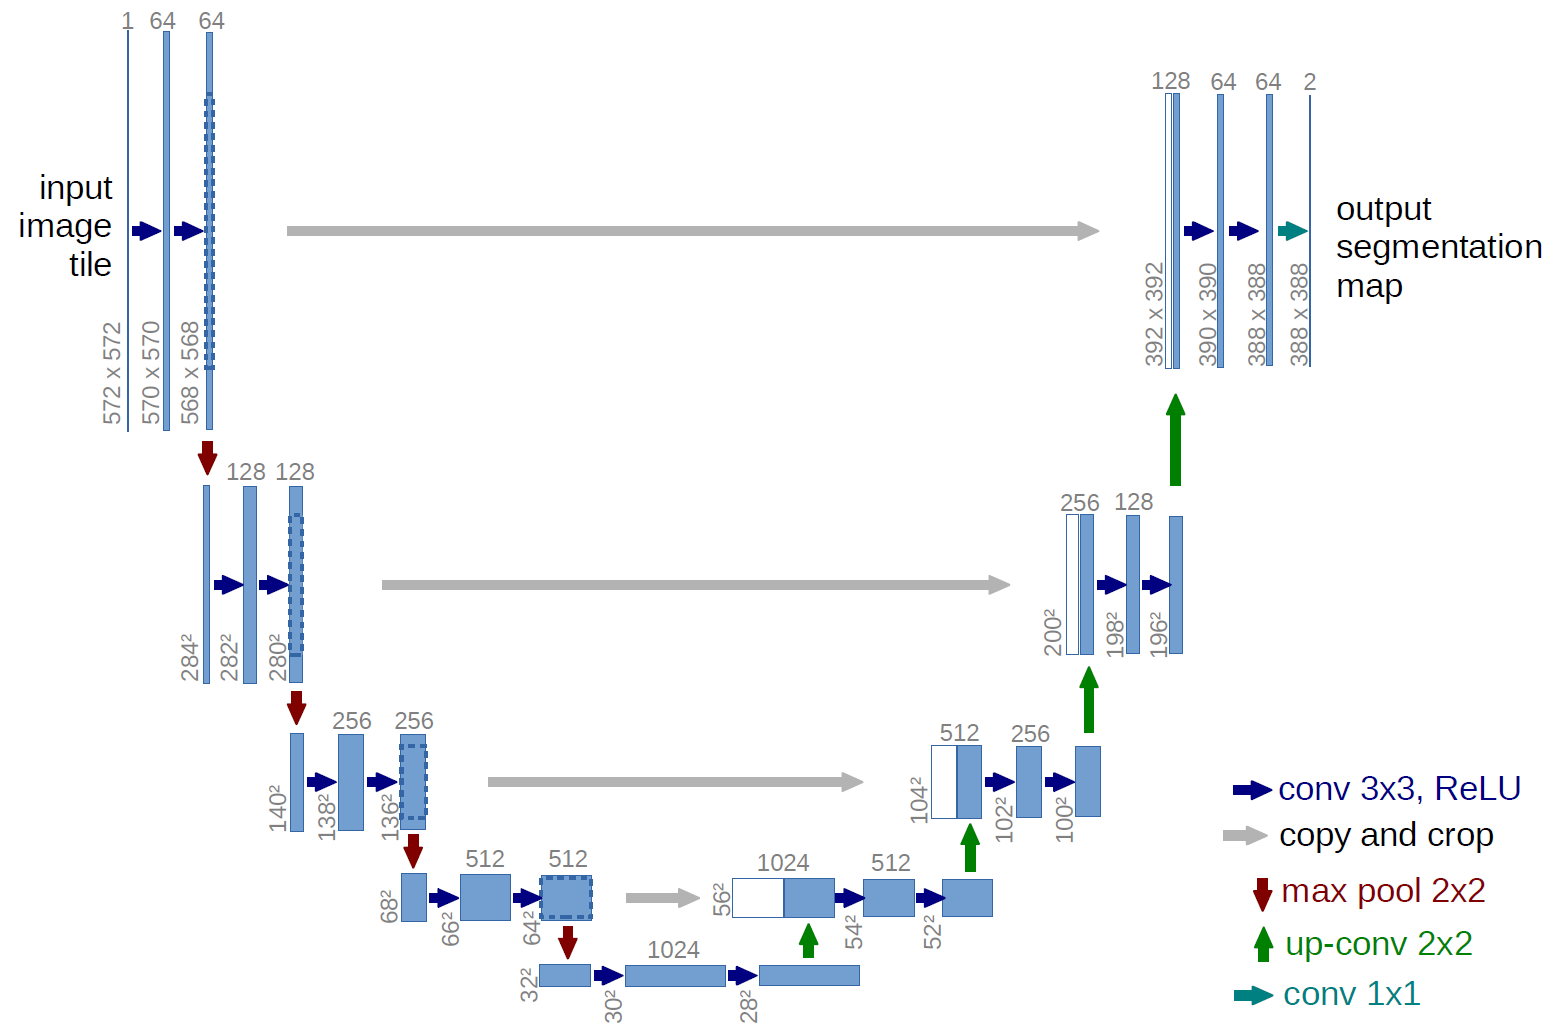
\includegraphics[width=0.8\textwidth]{Bilder/u-net-architecture.png} 
	\caption{Ursprüngliche U-Net-Architektur \cite{Ronneberger.18052015}.}
	\label{fig:u-net-architecture}
\end{figure} 

\section{Vortrainierte \ac{CNN}-Modelle} \label{sec:pretrained-backbones}

Im Folgenden wird eine Auswahl an \ac{CNN}-Modellen vorgestellt, von denen es öffentlich zugängliche,
vortrainierte Instanzen zur akademischen Verwendung gibt. Obwohl es sich um Klassifikationsmodelle handelt,
können die Modelle zu Transfer-Learning-Zwecken für semantische Segmentierung
genutzt werden, indem sie als \textit{Backbone} in den Encoder-Teil eines U-Net eingebaut werden 
(mehr dazu in \autoref{sec:transfer-learning}). \\ 
Die Klassifikations-Modelle sind auf dem Bildklassifikationsdatensatz \textit{ImageNet}, der über 14 Mio. Bilder 
mit 1000 Objektklassen enthält, trainiert. Der ImageNet-Datensatz ist der größte und bekannteste 
Datensatz seiner Art und ist sehr beliebt für Benchmarks und Pre-Training.

\subsection{VGG16} \label{sec:pretrained-backbones:vgg16}

\textit{VGG16} ist ein \ac{CNN}, welches 2015 von der \textit{Visual Geometry Group} vorgestellt wurde 
und zu der Zeit bahnbrechende Ergebnisse bei der Bilderklassifizierung lieferte \cite{Simonyan.04092014}. 
Inzwischen ist es ein Standard-Netz, auf welchem viele weitere Architekturen aufbauen,
um verschiedene Verbesserungen zu realisieren. 
Dadurch ist es auch sehr beliebt für Transfer-Learning. 

VGG16 besteht aus fünf Blöcken mit $3{\times}3$-Convolution-Schichten,
gefolgt von drei Fully-Connected-Schichten. Die ersten beiden Convolution-Blöcke haben zwei Convolution-Schichten,
die letzten drei Blöcke dagegen jeweils drei. 
Jeder Convolution-Block wird gefolgt von einer Maxpool-Schicht und jeder bis auf den vorletzten verdoppelt die Filteranzahl in den Convolution-Schichten,
beginnend bei 64 Filtern im ersten Block bis hin zu 512 Filtern in den letzten beiden Blöcken \cite{Simonyan.04092014}\footnote{\autoref{fig:vgg16-architecture} veranschaulicht VGG16.}. 

Das gesamte Netz besitzt 138 Mio. Parameter. Werden die drei Fully-Conntected-Schichten am Ende ausgelassen, 
sind es ungefähr 14,7 Mio. Parameter. 

\subsection{ResNet34} \label{sec:pretrained-backbones:resnet}

Damit Modelle mehr und feinere Features lernen können, müssen sie in der Lage sein, sehr komplexe Funktionen darzustellen. 
Das führt dazu, dass tiefere Netze auf dem ImageNet-Datensatz tendenziell bessere Ergebnisse erzeugen, als flachere. 
Hierin lag auch der Erfolg von VGG16 bzw. VGG19. Jedoch führt das einfache Vertiefen von Netzen zu dem Degredation-Problem, wonach 
flachere Netze besser performen, als tiefere, da die tieferen sehr schwer zu trainieren sind. \\
Dieses Problem adressiert \textit{ResNet} erfolgreich, indem \textit{Residual-Blocks} eingeführt werden. 
Hierdurch können mit \textit{ResNet} tiefere Netze erstellt werden als bisher, die trotzdem noch effizient trainiert werden können.
Ein Residual-Block besteht dabei aus zwei Convolutional-Layern mit einer Skip-Connection zwischen dem Input der ersten und dem Output 
der zweiten Layer. Durch die Skip-Connections kann bei der Backpropagation der Gradient ungehindert rückwärts laufen, 
um so auch die flachen Layer upzudaten. So kann z.B. \textit{ResNet34} 34 trainierbare Layer haben, 
während zuvor mit VGG nur 16 bzw. 19 effektiv waren \cite{He.10122015}. 

Die Architektur ist dabei sehr simpel. Sie stellt - im Falle von ResNet34 - 33 Convolutional-Layer mit wiederholtem Downsampling 
und Skip-Connections zwischen jeweils zwei Convoltuional-Layern, gefolgt von einer Fully-Connected-Layer dar \cite{He.10122015}\footnote{\autoref{fig:resnet34-architecture} veranschaulicht ResNet34.}.

ResNet34 hat 63,5 Mio. Parameter. Wird auf die letzte Fully-Connected-Layer verzichtet, sind es 21,2 Mio. Parameter.

\subsection{DenseNet121} \label{sec:pretrained-backbones:densenet121}

\textit{DenseNet121} wurde 2018 erstmals vorgeschlagen und designt, um das Vanishing-Gradient-Problem 
zu verbessern, bessere Feature-Übertragung in tiefere Netzschichten zu ermöglichen und das Wiederverwenden von Features 
zu unterstützen, um somit die Anzahl der benötigten Parameter bei gleichbleibender Performanz deutlich zu reduzieren \cite{Huang.25082016}.

Das Netz besteht aus mehreren sogenannten Dense-Blöcken, die wie folgt aufgebaut sind: 
Jede angegebene Convolution-Schicht besteht aus einer Batch-Normalization-Schicht mit \ac{ReLU}-Aktivierung,
gefolgt von der angegebenen Convolution-Schicht. Außerdem - und hier liegt die große Erweiterung des DenseNet - sind alle 
Convolution-Schichten eines Dense-Blocks mit allen nachfolgenden Convolution-Schichten des Dense-Blocks konkateniert,
anstatt nur mit dem einen Nachfolgenden, wie es zum Beispiel bei VGG16 der Fall ist\footnote{\autoref{fig:densenet121-architecture} veranschaulicht DenseNet121.}. 

DenseNet121 enthält circa 7,6 Mio. Parameter. Ohne die letzte Fully-Connected-Schicht sind es noch circa 6,9 Mio. 
Bei nur halb so vielen Parametern erreicht DenseNet121 leicht bessere Ergebnisse als VGG16 auf dem ImageNet-Datensatz 
(93\% ggü. 92\% Accuracy für ImageNet-Top-5) \cite{Huang.25082016}. 

\subsection{Vortrainierte CNN-Modelle als U-Net-Backbone} \label{sec:pretrained-as-unet-backbone}

Prinzipiell dienen die Convolution-Schichten aller in \autoref{sec:pretrained-backbones} beschriebenen, vortrainierten Backbone-Netze 
der Feature-Erkennung und -Extraktion. Lediglich die letzten Schichten, die bei den beschriebenen Klassifikationsmodellen  
Fully-Connected-Schichten waren, sind für die Zuordnung der Features zu den Objektklassen 
im ImageNet-Datensatz notwendig. Werden diese Schichten mit einem Decoder-Teil, der den Encoder - hier 
also das vortrainierte Klassifikationsnetz - spiegelt, ersetzt, entsteht ein Modell zur semantischen Segmentierung. 
Weiter müssen lediglich an geeigneter Stelle Skip-Connections zwischen Encoder und Decoder eingefügt werden,
um die U-Net-Form nachzubilden. 


\section{Transfer-Learning} \label{sec:transfer-learning}

\textit{Transfer-Learning} beschreibt das Übertragen von trainierten Gewichten eines \ac{ML}-Modells auf ein anderes, 
bestenfalls ähnliches Problem und Modell. Das Modell wird dann mit dem neuen Datensatz und unterschiedlichen Trainingsmethoden via \textit{Fine-Tuning} verfeinert.
Häufig wird dafür ein Teil des Modells eingefroren, sodass sich die eingefrorenen Gewichte nicht verändern können. Dies verhindert, 
dass die bereits vortrainierten Gewichte durch die erste Trainings-Batch ruiniert und unbrauchbar werden. Eine weitere Möglichkeit ist,
mit einer sehr geringen Lernrate das gesamte Modell zu trainieren. Oft werden beide Ansätze auch verbunden.

Der Vorteil von Transfer-Learning liegt darin, dass das Training deutlich kürzer dauert, 
weil direkt mit einer höheren Genauigkeit eingestiegen wird, mit kleineren Datensätzen bessere Ergebnisse erzielt werden können
 und auch insgesamt eine höhere Genauigkeit 
am Ende des Trainings erreicht wird, als bei herkömmlichem Training. Diese Effekte sind verstärkt, 
abhängig davon, wie ähnlich der Datensatz des Pre-Trainings und des eigentlichen Trainings sind \cite{Ruder.3212017}. \\
Insbesondere bei Computer-Vision ist Transfer-Learning effektiv, da sich bei Bildern high-level Features wie Clustering 
ähnlichfarbiger Pixel oder Kantenerkennung kaum unterscheiden zwischen unterschiedlichen Datensätzen und damit bereits vorhanden sind \cite{Ruder.3212017}. 

Für Transfer-Learning mit U-Nets gibt es verschiedene Strategien: Backbone-Netze als Encoder, 
partielles Einfrieren verschiedener Netzbereiche und direktes Trainieren mit geringer Learning-Rate.

Zunächst ist im Kontext von Transfer-Learning bei U-Nets ein \textit{Backbone} ein etabliertes vortrainiertes \ac{CNN}, 
welches, leicht modifiziert, als Encoder für das U-Net verwendet wird. Hierbei wird der Decoder-Teil des U-Net 
symmetrisch dem Encoder nachempfunden und an passenden Stellen Skip-Verbindungen zwischen En- und Decoder eingebaut. \\
Hierdurch kann eine geeignete \ac{CNN}-Architektur für das spezifische Problem ausgewählt werden. Des Weiteren sind diese 
Modelle auf sehr großen Datensätzen, wie \textit{ImageNet}, vortrainiert öffentlich zugänglich. 

Das Fine-Tuning kann unterschiedlich ablaufen, so wurden beispielsweise bei der
semantischen Segmentierung von medizinischen Lungen-Ultraschall-Bildern die besten Ergebnisse  
mit einem U-Net mit auf ImageNet trainierten \textit{VGG16}-Backbone erzielt. Das Vergleichsnetz, welches auf einem weniger umfangreichen
Datensatz (der \textit{Salient-Objects}-Datensatz) vortrainiert wurde, erzielte schlechtere Ergebnisse in Bezug auf das Dice-Maß, wobei allerdings das VGG16-U-Net kleine falsch-positive 
Regionen erkannte \cite{Cheng.05.10.2021}. \\
Das Netz mit VGG16-Backbone wurde fine-tuned, indem der Encoder eingefroren wurde und nur der Decoder trainiert.
Das Fine-Tuning auf dem Vegleichsnetz wurde auf zwei Weisen durchgeführt: 
\begin{enumerate}
	\item Ohne Einfrieren, mit einer Lernrate von $10^{-5}$ und
	\item mit Einfrieren des mittleren Blocks, welcher ungefähr $14\cdot 10^6$ der insgesamt $31 \cdot 10^6$ Parameter enthielt. 
\end{enumerate}
Hierbei erzielte das Vergleichsnetz deutlich bessere Ergebnisse bei Training mit geringer Lernrate und ohne Einfrieren \cite{Cheng.05.10.2021}.

In einem weiteren Paper wurde untersucht, welche Layer eines U-Net am besten eingefroren werden sollten, für das Fine-Tuning von medizinischen Bildern - 
zum einen von Lungen-Ultraschall-Bildern und zum anderen von Brust-Röntgen-Aufnahmen. 
Hier wurde wieder mit dem \textit{Salient-Objetcs}-Datensatz vortrainiert. Dann wurden für beide Anwendungsfälle folgende Tests durchgeführt: 
\begin{enumerate}
	\item Einfrieren der linken Hälfte (Encoder) des Netzes,
	\item Einfrieren der rechten Hälfte (Decoder) des Netzes,
	\item gesamtes Netz, bis auf den ersten Block eingefroren und dann nach jeweils fünf Epochen sukzessive weitere Blöcke freigeben und
	\item dasselbe allerdings von hinten nach vorne.
\end{enumerate}
Für die Röntgenaufnahmen gab es keine Unterschiede zwischen den Methoden. \\
Für die Ultraschallbilder lieferte Methode (1) die schlechtesten Ergebnisse (Dice: $0.72$), gefolgt von Methode (2) (Dice: $0.80$) 
und gleichermaßen (3) und (4) (Dice: $0.82$) \cite{Amiri.19.02.2020}. 

Es ist ersichtlich, dass die Methodik beim Fine-Tuning, abhängig vom Datensatz, dem Anwendungsproblem und dem vortrainierten Backbone, einen erheblichen Einfluss 
auf die abschließende Performanz des Modells haben kann aber nicht muss. 
Um das Netz also zu optimieren und die besten Ergebnisse zu erzielen sollte also neben den Hyperparametern die Fine-Tuning-Methode untersucht werden. 
Die hier vorgestellten Methodiken können später genutzt werden, 
um eine Transfer-Learning-Methode für das Problem der Radwegerkennung zu konzipieren. 


\section{Aktueller Stand bei der Straßendetektion}

Die Erkennung von Fahrradwegen soll auf der bereits existierenden Straßenextraktion aus Luftbildern aufbauen.
Hierfür werden vorhandene Datensätze für Straßen vorgestellt. 
Im Anschluss werden auf den aktuellen Stand und Benchmark-Optionen eingegangen.

\subsection{Datensätze} \label{sec:road-detection:roads-data}

Im Folgenden sind relevante Datensätze zur Straßenerkennung aus Luftbildern aufgeführt. 
Eine Auswahl der später zum Pre-Training verwendeten Datensätze findet im \autoref{sec:pre-training-roads} statt.\\
Im Folgenden wird der Begriff \textit{Testdatensatz} verwendet, was hier einen sehr kleinen Datensatz, 
der ausschließlich zum Testen und Bewerten eines bereits 
trainierten Modells verwendet werden soll und ausschließlich dafür annotiert wurde, beschreibt 
und nicht den \textit{Test-Split} eines größeren Datensatzes. 
Im Rahmen der Straßenerkennung ist dies besonders relevant, 
da sich unterschiedliche Städte in unterschiedlichen Ländern und Kulturen stark unterscheiden können, 
während die Trainingsdaten meist nur aus einer Stadt, die in sich ein eher homogenes Bild aufweist, bestehen.
Der Testdatensatz soll also die Generalisierungsfähigkeit des Netzes testen, um zu identifizieren,
ob das Modell, das bspw. auf einem Datensatz einer modernen amerikanischen Stadt trainiert wurde, 
auch auf Bildern einer mitteleuropäischen Altstadt funktioniert. Deswegen ist es wichtig, 
dass keine Bilder des Testdatensatzes im Training verwendet werden. 

% Bei den letzten Datensets zu Toronto, Vaihingent und Potsdam handelt es sich um Testdatensätze. 
Beim \textit{Massachusetts Roads Dataset} liegen $1171$ Luftaufnahmen aus dem Gebiet Massachusetts vor.
Jedes der Bilder besteht aus $1500{\times}1500$ Pixeln, was einer Fläche von $2.25 km^2$ entspricht.
Ein Beispiel hiervon zeigt \autoref{fig:mass-example}.
Die gesamte Abdeckung sind $2600 km^2$ bestehend aus städtischer und ländlicher Gegend.
Der Split erfolgt im Verhältnis $95:1:4$. 
Über den Split wird sichergestellt, dass keine Durchmischung der Test- und Validierungsdaten mit den Trainingsdaten erfolgt und die Bewertung des Netzes verfälscht wird.
Es gibt also $1108$ Trainings-, $14$ Validierungs- und $49$ Testbilder.
Die Zielbilder sind über eine Rasterung der Straßenmittellinien aus dem \ac{OSM}-Projekt generiert worden.
Die Liniendicke der gelabelten Straßen beträgt $7 px$ und ist ungeglättet, da hiermit bessere Ergebnisse erzielt worden sind \cite{Mnih.2013}.
Der Zuschnitt der Bilder sorgt teilweise für einen hohen Anteil weißer Stellen in den Bildern.

\begin{wrapfigure}{r}{0.50\textwidth}
	\centering
	\vspace{-20pt} % Manchmal möchte man den oberen Abstand selbst anpassen
	\includegraphics[width=0.45\textwidth]{Bilder/mass_example.png}
	\vspace{-5pt}
	% Das folgende ist ein Trick, um "Abbilgung x.y" in eine
	% eigene Zeile zu packen. Der Text zwischen [ und ] steht
	% im Abbildungsverzeichnis. Der Text darunter wird
	% tatsächlich angezeigt.
	\caption[$1500{\times}1500$-Pixel Beispiel des Massachusetts-Datensatzes.]{\unskip}
	$1500{\times}1500$-Pixel Beispiel des Massachusetts-Datensatzes.
	\label{fig:mass-example}
\end{wrapfigure}

Das \textit{Buffalo Roads Dataset} ist als zusätzliches Testset für das Massachusetts Roads Dataset zu sehen.
Hintergrund ist die Überprüfung des Netzes mit Daten aus einem anderen Gebiet unter anderen Bedingungen.
Es besteht lediglich aus 30 Fotos ($5:5:20$) mit einer Größe von $609{\times}914$ und einer Auflösung von $1 \frac{px}{m^2}$.
Die Generierung der gelabelten Daten erfolgt analog zum Massachusetts Road Dataset über \ac{OSM}.
Größter Unterschied ist die Verdeckung von Straßen durch Bäume \cite{Mnih.2013}.

\textit{LandCover.ai} kann für die Erkennung von Gebäuden, Waldgebieten, Gewässern und Straßen verwendet werden.
Die Aufnahmen stammen aus Polen und Zentraleuropa in einer Größe von $21627 km^2$.
$33$ Bilder haben eine Auflösung von $25 \frac{cm}{px}$ mit $9000{\times}9500$ Pixeln und 
$8$ Bilder von $50 \frac{cm}{px}$, mit $4200{\times}4700$ Pixeln.
Die Bilder sind hand-annotiert und beinhalten einen großen Anteil an ländlichen Gebieten \cite{.20.04.2022}.

Mithilfe des \textit{Deep Globe Road Extraction Datasets} können in Katastrophengebieten Informationen über Karten und Zugänglichkeitsmöglichkeiten für die Krisenbewältigung gesammelt werden.
Der Datensatz besteht aus $6226$ Luftbildern in RGB, mit einer Größe von $1024{\times}1024$.
Die Auflösung der Aufnahmen beträgt $50 cm$. \autoref{fig:deep_globe-example} zeigt ein Beispiel.
Mit $1243$ Validierungs- und $1101$ Testdaten ist der Split in Training, Validierung und Test zu $73:15:13$ erfolgt.
Der hohe Aufwand zur Erstellung der Labels führt zu Ungenauigkeiten, insbesondere in ländlichen Regionen. 
Kleine Straßen innerhalb von Landwirtschaftsflächen sind bewusst unbeschriftet geblieben.
Die Bilder sind ursprünglich über Thailand, Indonesien und Indien, mit je $19584{\times}19584$ Pixeln aufgenommen worden.
Insgesamt entspricht es einer Fläche von $2220~km^2$ \cite{Ashwath.10.11.2020}.

\begin{wrapfigure}{l}{0.5\textwidth}
	\centering
	\vspace{-0pt} % Manchmal möchte man den oberen Abstand selbst anpassen
	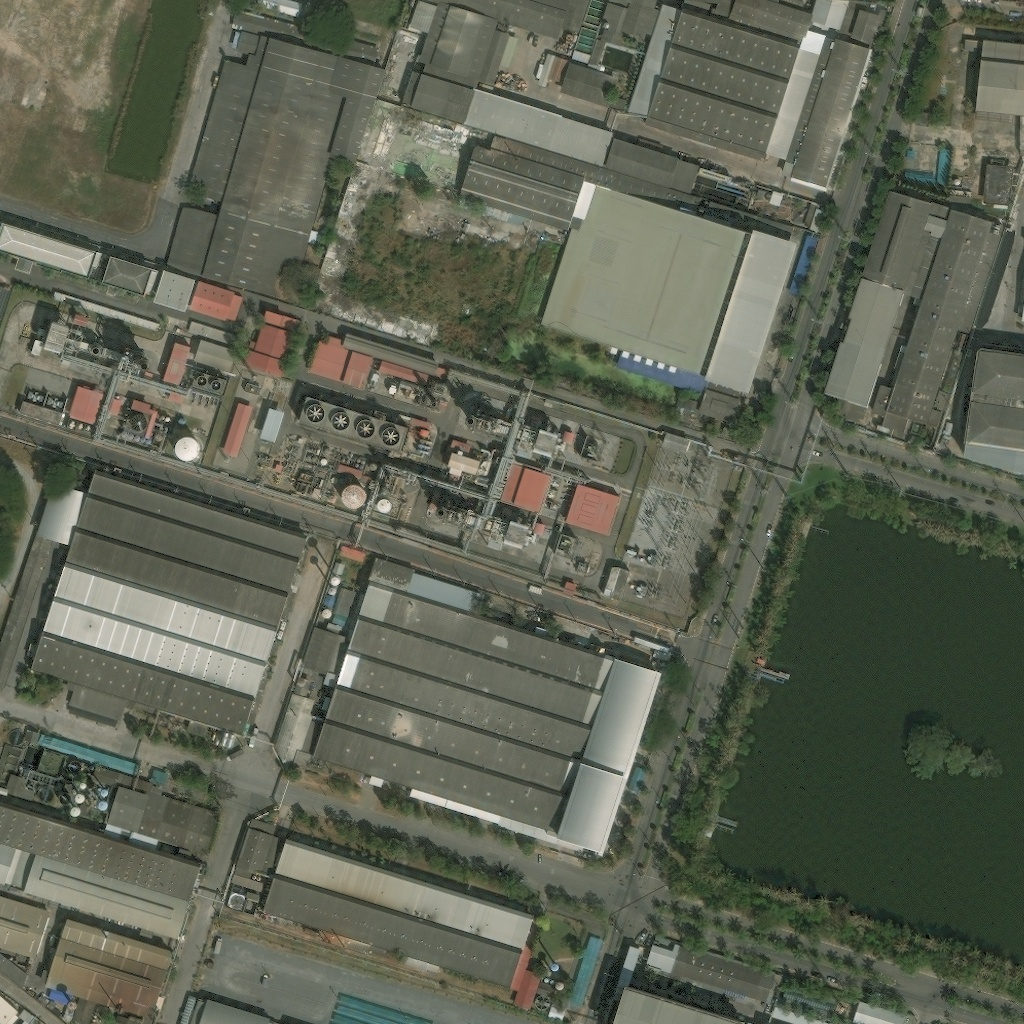
\includegraphics[width=0.45\textwidth]{Bilder/deep_globe_example.jpg}
	\vspace{-5pt}
	% Das folgende ist ein Trick, um "Abbilgung x.y" in eine
	% eigene Zeile zu packen. Der Text zwischen [ und ] steht
	% im Abbildungsverzeichnis. Der Text darunter wird
	% tatsächlich angezeigt.
	\caption[$1024{\times}1024$-Pixel Beispiel des Deep-Globe-Datensatzes.]{\unskip}
	$1024{\times}1024$-Pixel Beispiel des Deep-Globe-Datensatzes.
	\label{fig:deep_globe-example}
\end{wrapfigure}

Bei den nachfolgenden drei Datensätzen handelt es sich um Testdatensätze.
Das \textit{Toronto Dataset} umfasst $1,45km^2$ im Umkreis der Stadt Toronto in Canada. 
Darin enthalten sind ca. $1 km$ Straßen mit einer Bodenauflösung von $15cm$. 
Zusätzlich werden Laserscanner mit $6 \frac{points}{m^2}$ bereitgestellt.
Im Datensatz ist eine hohe Varianz bezüglich der Gebäudehöhe, Struktur der Dächer und verschiedener Straßen vorzufinden.
Der Testbestand kann für die Überprüfung von Objektextraktion und Gebäuderekonstruktionstechniken in zwei weitere Teilgebiete unterteilt werden.
Für Straßen können alle Testdaten verwendet werden.
Die Labels sind manuell mithilfe von CloudCompare erstellt worden \cite{Englich.06.10.2022b,Tan.2020}.

Der Testdatensatz \textit{Vaihingen/Enz} besteht aus einer Untermenge der Daten, welche für einen Test von digitalen Luftbildkameras verwendet wurden.
Er ist in drei Testgebiete für verschiedene Objektklassen und in einen größeren Bereich für das Überprüfen von Straßenextraktion aufgeteilt, wobei die drei Gebiete hier mit inbegriffen sind.
Die einzelnen Gebiete sind in verschiedene Kategorien unterteilt: Hochhäuser, Wohngebiete mit kleineren Einfamilienhäusern und Innenstadt mit dichter Bebauung.
Die Bodenauflösung beträgt $8cm$ \cite{Englich.06.10.2022b}.

Für die Stadt \textit{Potsdam} gibt es einen ähnlichen Datensatz. 
Dieser zeigt eine typische Altstadt mit großen Gebäudeblöcken, kleinen Straßen und einer dichten Besiedelung.
Die \ac{GSD} beträgt $5cm$.
Zur Vermeidung von Randbereichen ohne Daten sind zentrale Ausschnitte verwendet worden.
Übrig gebliebene Datenlücken wurden interpoliert \cite{Englich.17.11.2022}.

\subsection{Aktueller Stand und Benchmarks} \label{sec:state-of-the-art-roads} % ...der straßen detection

Die aktuellen State-Of-The-Art-Methoden zur Extraktion von Straßen aus Satelliten- und Luftbildern verwenden 
alle Computer-Vision mittels \acp{CNN} und dabei ausschließlich Netze aus der U-Net-Familie - also angepasste, 
erweiterte, abgeänderte U-Nets \cites{C.Henry.2021, Constantin.2018, Kamiya.2018, Yerram.2022}. \\
Dies liegt vor allem daran, dass das U-Net, welches ursprünglich für biomedizinische Bilder entworfen wurde, 
genau die Probleme adressiert, die auch beim Segmentieren von Straßen auf Luftbildern auftreten. 
Wie auch in medizinischen Bildern leiden die Luftbilder-Datensätze häufig unter großer Klassen-Imbalance 
und unter ähnlichen Annotationsfehlern. Außerdem haben viele medizinische Bilder und Luftbildaufnahmen von Straßen 
ähnliche Topologien. Komplexere Architekturen zur semantischen Segmentierung, wie zum Beispiel solche 
für Bodenaufnahmen-Datensätze (vgl. KITTI \cite{Geiger.2013}) erreichen nicht die Performance von U-Nets bei 
Luftbild-Benchmarks \cite{C.Henry.2021}. \\
Weiter wird die Extraktion von Straßen aus Satelliten- bzw. Luftbildern zumeist in zwei Phasen eingeteilt: 
\begin{enumerate}
	\item das Erstellen einer binären Maske zu den Luftbildern mittels semantischer Segmentierung, 
	welche die Straßen pixelweise induziert, 
	\item das Extrahieren eines topologischen Graphens, welcher die Straßen-Zentrumslinien beschreibt.   
\end{enumerate}
Schritt (1) wird dabei zumeist von U-Net-Derivaten behandelt, wobei es allerdings auch Vorschläge von Netzen gibt, 
die direkt Schritt (2) ausführen \cite{C.Henry.2021}.
Im Folgenden wird weiter Schritt (1) betrachtet.   

Der Vergleich von unterschiedlichen Netzen, Papern und Ergebnissen zur Straßenerkennung ist häufig erschwert, 
da es trotz gleicher Bewertungsmaße wie Dice oder \ac{IoU}, zwei unterschiedliche gängige Kodierungen gibt:
\begin{enumerate}
	\item Das verwendete \ac{CNN} hat je Input-Neuron bzw. -Pixel $p$ genau ein Output-Neuron $o_p$, welches den jeweiligen Input-Pixel $p$
	als Straße identifiziert, genau dann, wenn der Wert des Output-Neuron $o_p$ einen gewissen Grenzwert $l$ überschreitet ($o_p > l$), 
	ansonsten ($o_p \leq l$) gilt der Pixel $p$ \textit{implizit} als Nicht-Straße, bzw. \textit{Hintergrund}. \\
	In diesem Fall stellt ein korrekt als Hintergrund klassifizierter Pixel ein wahr-negatives Ergebnis dar. 
	Wahr-Negative werden von Dice, bzw. \ac{IoU} allerdings nicht berücksichtigt (vgl. \autoref{eq:f1} und \ref{eq:iou-binary}).
	Ein so klassifizierter Pixel ändert also nichts an dem Score. Es werden nur Straßen betrachtet, nicht aber der Hintergrund.    
	\item Das verwendete \ac{CNN} hat je Input-Neuron bzw. -Pixel $p$ \textit{zwei} Output-Neuronen $\mathbf{o_p} = (o_{p_S}, o_{p_H})$, 
	wobei dies eine One-Hot-Kodierung von Punkt (1) darstellt. 
	Ein Hintergrundpixel wird nun \textit{explizit} als solcher klassifiziert. 
	Dies ändert allerdings die Berechnungsgrundlage von Dice und \ac{IoU} erheblich, da diese indessen (zumeist) als Mittelwert 
	der Scores zu $o_p{_S}$ und $o_p{_H}$ berechnet werden. Hierdurch fließen die zuvor unberücksichtigten wahr-negativen 
	Hintergrundpixel als wahr-postive in den Dice- bzw. \ac{IoU}-Score ein. Die Verzerrung wird noch verstärkt, 
	da eine starke Imbalance zwischen Straßen- und Hintergrundpixel herrscht, wodurch der Dice-/\ac{IoU}-Score bei 
	der One-Hot-Kodierung viel mehr eine Aussage darüber trifft, wie viele Hintergrundpixel, von denen es ja viel mehr gibt,
	richtig klassifiziert wurden. Die so erzielten Dice-/IoU-Werte sind hier rein numerisch deutlich höher. 
\end{enumerate}
\autoref{fig:problematic-output} visualisiert das Problem der Vergleichbarkeit von Dice/IoU je nach gewählter Output-Kodierung.
Das Problem verstärkt sich bei mehr Pixeln. Im Beispiel wurde die Hälfte aller Straßen korrekt erkannt, 
weswegen eine IoU von 50\% zu erwarten ist. Liegt jedoch eine One-Hot-Kodierung vor, werden 75\% aller Pixel richtig erkannt.
Dies spiegelt allerdings nicht die Empirie wider, da kein Interesse an korrekt klassifizierten Hintergrundpixeln besteht.
Durch die One-Hot-Kodierung kommen bei manchen Modellen zur Straßenerkennung IoU-Werte von über 95\% zu Stande.
Im Weiteren wird für alle Werte eine implizite Kodierung (50\% in \autoref{fig:problematic-output}) vorausgesetzt. 

\begin{figure}
	\centering
	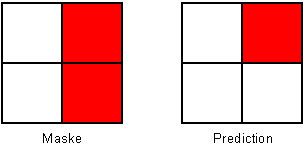
\includegraphics[width=0.5\textwidth]{Bilder/output-enc-example.drawio.pdf} 
	\vspace{-5pt}
	\caption{Veranschaulichung des Problems der Output-Kodierung. Links zeigt die 4-Pixel-Ground-Truth-Maske, 
	wobei weiße Flächen Hintergrund und rote Straße darstellen. Rechts zeigt die semantische Segmentierung 
	eines Modells, wobei der Pixel rechts unten fälschlicherweise als Hintergrund klassifiziert wurde.
	Bei einer impliziten Kodierung mit einem Output ist $IoU = 50\%$, bei einer One-Hot-Kodierung ist $IoU = 75\%$.}
	\label{fig:problematic-output}
\end{figure} 

Im Weiteren werden aktuelle Ergebnisse zu den Massachusetts- und Deep-Globe-Datensätzen vorgestellt, 
um zu ermitteln, was für diese Datensätze gut funktioniert, sodass diese state-of-the-art Erkenntnisse beim 
späteren Entwurf eines oder mehrerer Netze zum Erkennen von Fahrradwegen (s. \autoref{sec:architecture}) 
genutzt werden können. Die beiden Datensätze sind für die Literaturrecherche ausgewählt, 
da sie sehr häufig als Benchmark zum Erkennen von Straßen genutzt werden, es dazu sehr viel Literatur und 
Forschung gibt und da beide Datensätze sich stark unterscheiden, soweit das im Rahmen der Straßenerkennung möglich ist. 
Haben die State-Of-The-Art-Lösungen trotz des starken Unterschieds der Datensätze ähnliche gut funktionierende
Komponenten, stärkt das die Annahme, dass diese Komponenten auch für das Erkennen von Radwegen nützlich sein könnten. 

\begin{table}[H]
	\centering
	\begin{tabular}{l|l|l|l|l}
		\multirow{2}{*}{Model} & \multicolumn{2}{c|}{Massachusetts} & \multicolumn{2}{c}{Deep Globe}  \\
		& Dice & IoU & Dice & IoU \\
		\midrule
		DeepLabv3+* & 69,35 & 52,95 & 75,19 & 59,65 \\
		D-LinkNet50 & 71,01 & 54,90 & 74,04 & 58,12 \\
		U-Net* & 71,91 & 55,92 & 76,82 & 61,97 \\
		Res-U-Net50 & 72,74 & 56,93 & 78,62 & 64,55  \\
		Dense-U-Net-121 & \textbf{73,03} & \textbf{57,12} & \textbf{79,19} & \textbf{65,13}  \\
	\end{tabular}
	\caption{Baseline-Resultate verschiedener Modelle auf dem Massachusetts- 
	bzw. Deep-Globe-Datensatz in Prozent, aufsteigend sortiert. Nicht one-hot-kodiert. \\ * nicht vortrainiert \cite{C.Henry.2021}.}
	\label{tab:basline-benchmarks}
\end{table}

\autoref{tab:basline-benchmarks} zeigt Resultate zum Massachusetts- und Deep-Globe-Datensatz von sogenannten \textit{Baseline}-Modellen.
Hierbei handelt es sich um verschiedene Architekturen, die allerdings nicht sonderlich auf den jeweiligen Datensatz optimiert sind,
was die Hyperparameter oder manche Architektur-Anpassungen angeht. Ein Beispiel dafür wäre das Ausprobieren von verschiedenen (Kompositions-)Kostenfunktionen. 
Mit den Baseline-Resultaten können diese Modelle zu Vergleichszwecken verwendet werden 
und es bestehen Daten zu mehreren Benchmarks. Aus den Baseline-Resultaten lässt sich schließen, dass das Vortrainieren eines Netzes auf einem 
anderen Datensatz bessere Ergebnisse für die Straßendatensätze und somit ggf. auch für die spätere Betrachtung mit 
den Radweg-Datensätzen liefert \cite{C.Henry.2021}.

\newcommand*\rot{\rotatebox{60}}

\begin{table}
	\centering
	\begin{tabular}{r|l|l}
		& Modell & IoU \\
		\midrule
		& RDRCNN & \textbf{67,10} \\
		Massachusetts & Dense-U-Net-121 & 66,61  \\
		& WRAU-Net & 64,58 \\
		\midrule
		& EOSResUNet & \textbf{65,60} \\
		Deep Globe & D-LinkNet & 64,12 \\
		& U-Net-likeResNet34 & 64,00 \\
	\end{tabular}
	\caption{Optimierte Resultate verschiedener Modelle auf dem Massachusetts- 
	bzw. Deep-Globe-Datensatz in Prozent, absteigend sortiert. Nicht one-hot-kodiert \cite{C.Henry.2021}.}
	\label{tab:optimized-benchmarks}
\end{table}


\autoref{tab:optimized-benchmarks} zeigt hingegen die top-drei optimierten Modelle, die derzeit die Leaderboards 
des jeweiligen Datensatzes anführen. Alle hiervon sind U-Net-Derivate.
Mit der Modell-Optimierung kann \textit{Dense-U-Net-121} aus \autoref{tab:basline-benchmarks} beispielsweise beim Massachusetts-Datensatz 
bis zu 66,61\% erreichen, anstelle von den 57,12\% wie im Baseline-Fall. 
Dense-U-Net-121 ist dabei ein U-Net mit einem vortrainierten DenseNet121 als Backbone \cite{C.Henry.2021}. \\
Im Falle vom RDRCNN (Refined Deep Residual Convolutional Neural Network), konnte die große Verbesserung erzielt werden,
indem das U-Net so angepasst wurde, dass die Encoder-Blöcke mit Residual-Blöcken\footnote{Zwei Convolutional-Layer bei dem eine Skip-Connection zwischen dem Input der ersten und dem Output der zweiten Schicht besteht (s. \autoref{sec:pretrained-backbones:resnet}).} 
ersetzt wurden und der Bottleneck-Block
um Dilatation erweitert wurde \cite{Gao.2019}. 
Beim EOSResUNet wurden ebenfalls die Encoder-Blöcke mit Residual-Blöcken ersetzt und zusätzlich nach \ac{IoU} statt nach Dice oder \ac{BCE} optimiert \cite{O.Filin.2018}. \\
Die besten Netze beider Datensätze haben die Gemeinsamkeit der U-Net-Struktur, wie auch die Residual-Blöcke (bzw.
sogar Dense-Blöcke, was als eine Erweiterung der Residual-Blöcke aufgefasst werden kann). 
Diese Informationen können zur Konzeption eines Netzes zur Radwegerkennung verwendet werden.  

\section{Neuheitswert} \label{sec:novelty}

Aus der vorangegangenen Betrachtung des Stands der Technik ergeben sich drei neuartige Probleme, die 
diese Arbeit untersucht:
\begin{enumerate}
	\item Bisher existieren keine wissenschaftlichen Untersuchungen, die versuchen, unterschiedliche Straßenelemente,
	wie Gehwege, Radwege, Busspuren o.Ä. auf Luftaufnahmen von Straßen zu unterscheiden. Da Straßen als Ganzes 
	auf Luftbildern gut zu erkennen sind, deren unterschiedliche, sehr heterogenen Bestandteile jedoch weniger, 
	kann mit dem Beispiel der Radwege überprüft werden, ob die Unterscheidung mit derzeitigen Luftbildqualitäten von circa 20 bis 50 cm \ac{GSD} 
	möglich ist. 
	\item Da für vorgenannten Punkt noch keinen Datensatz vorhanden ist, muss ein solcher erstellt werden. Dieser muss umfangreich 
	genug sein, dass er für \ac{ML} verwendbar ist. Es soll geklärt werden, ob bisherige Methoden, Datensätze für die Straßenerkennung 
	((semi-)automatisch) zu erstellen, auch für Radwege angewandt werden können und wie die Güte eines solchen Datensatzes bewertet werden kann. 
	\item Die Literatur bezüglich der Straßenerkennung fordert eine sehr genaue Segmentierung des Bildes. Für Radwege ist es ausreichend, 
	zu ermitteln, ob einer existiert und wo dieser grob liegt (auf welcher Straßenseite). Für diesen Verwendungszweck gibt 
	es auch ein Bewertungsmaß -- die \textit{Quality} (vgl. \autoref{sec:evaluation-metrics:quality}). Für die Quality gibt es allerdings
	keine Implementation auf Rastern, wie bei einer semantischen Segmentierung, sondern nur auf daraus extrahierten Graphen. 
	Folglich soll diese Arbeit eine Berechnungsmethode konzipieren, um die Quality auf die Masken der semantischen Segmentierung anzuwenden 
	(s. \autoref{sec:eval:biou} \textit{BIoU}), also einen Schritt bevor aus der Maske die Graphen extrahiert werden.  
	\item Da zum Pre-Training Datensätze zum Einsatz kommen, die keine deutschen Städte darstellen, 
	die Optik der Infrastrukturen sich in unterschiedlichen Ländern aber unterscheidet, kann diese Arbeit 
	Aufschluss darüber geben, ob Ergebnisse zwischen Städten unterschiedlicher Länder übertragbar sind.     
\end{enumerate} 